% !TeX root = ../../main.tex

\section{内存管理}

这一节讨论堆上的内存数据(在本文中只有向量这一种数据类型)以及如何管理堆内存。

堆内存与过程调用栈相互区分开,栈上的数据在函数退出后就无法再被访问了。
而堆允许我们通过引用来在不同的代码之间访问运行时创建的数据。
也正因此,堆上的数据的生命周期是不确定的。

\begin{lstlisting}
(let ([v (vector (vector 44))])
  (let ([x (let ([w (vector 42)])
             (let ([_ (vector-set! v 0 w)])
               0))])
    (+ x (vector-ref (vector-ref v 0) 0))))
\end{lstlisting}

例如在上面这个例子中,变量 w 的生命周期在绑定完 x 后就结束了,
但它指向的向量在这之后仍然可以被访问到,
因此上面这段代码的结果是0和42相加,也就是42。
我们在前一节讨论闭包时也使用了单元素向量来延长自由变量的生命周期。

从程序员可观察行为的角度来看,向量永远存在。
当然,如果它们真的永远存在,堆将越来越大,最终耗尽内存。
我们的语言必须实现自动地清理那些肯定不会再用到的数据,也就是垃圾回收。

\subsection{垃圾回收算法}

本文使用的是一个较为简单的垃圾回收算法:双空间拷贝回收\cite{Wilson_1992}。
图\ref{fig:copying-collector}给出了在垃圾回收之前(上面)和之后(下面)的内存情况。
在双空间收集器中,堆分为两个部分,分别命名为 FromSpace 和 ToSpace 。
最初,所有向量都分配到 FromSpace,当某次分配请求发现剩余的空间不够时,回收器开始工作。

\begin{figure}[t]
\centering
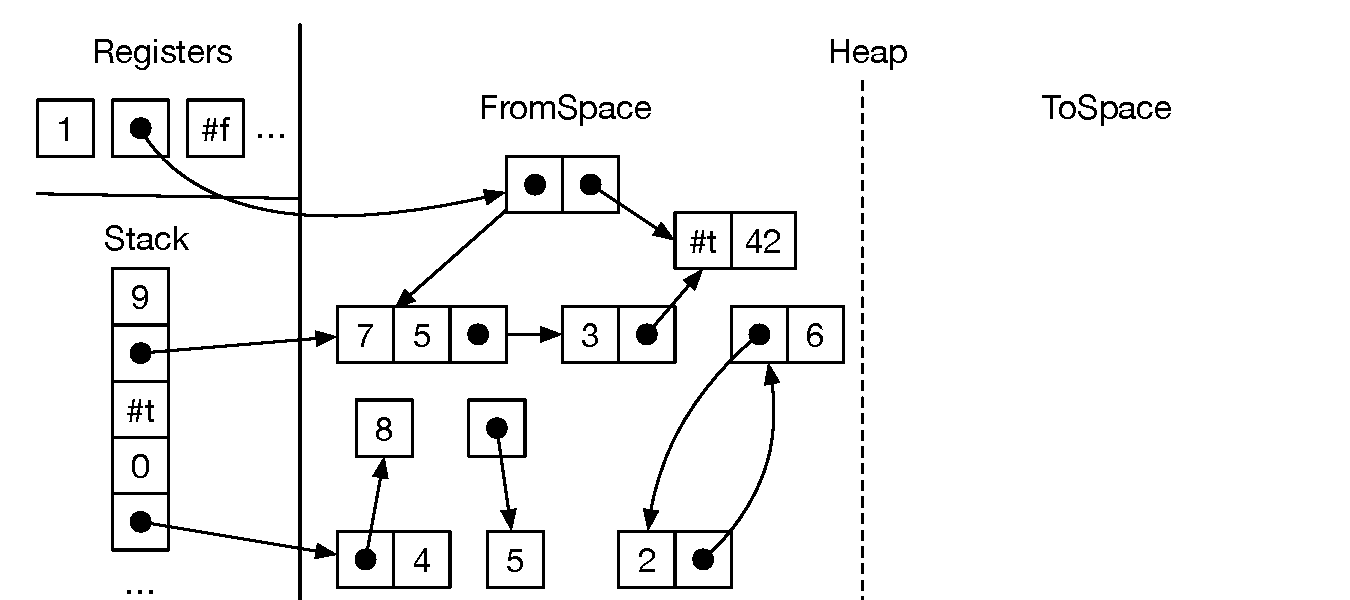
\includegraphics[width=\textwidth]{figures/copy-collect-1} \\[5ex]
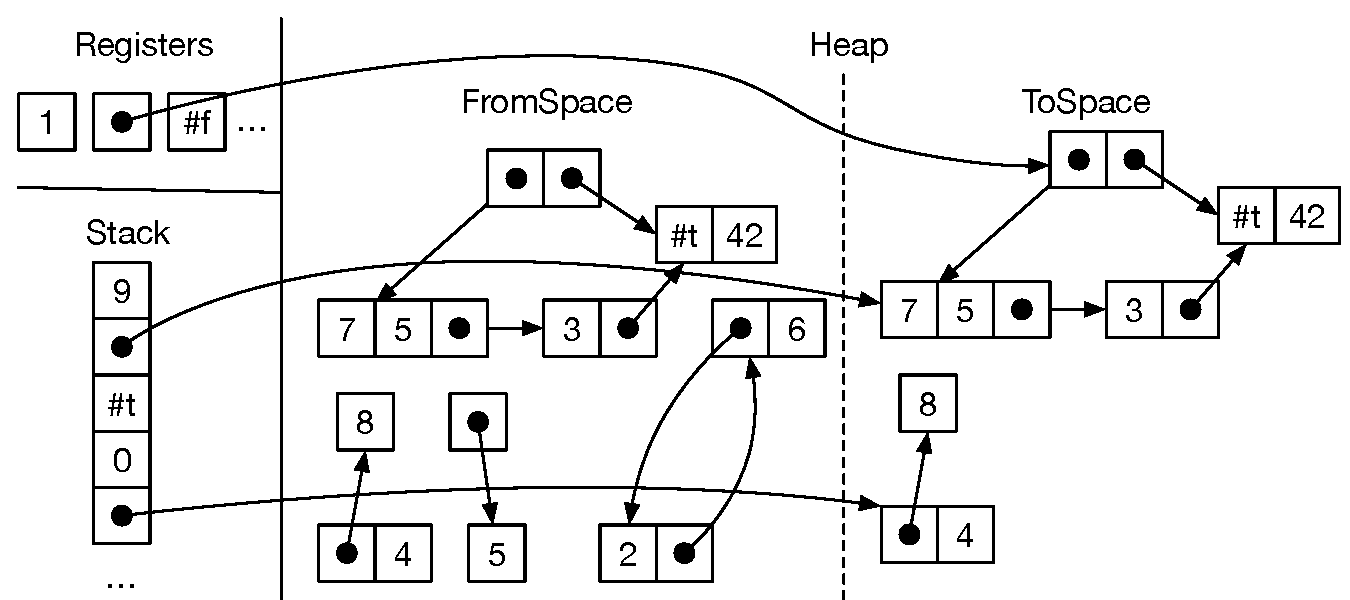
\includegraphics[width=\textwidth]{figures/copy-collect-2}
\caption{双空间拷贝回收示意图}
\label{fig:copying-collector}
\end{figure}

由于程序的行为是无法预知的,我们不可能准确地知道哪些向量在以后会被使用,哪些是垃圾。
但是我们可以保留下从当前所有变量出发,能访问到的那些向量,它们可能会被使用,也可能不会,
但剩余的不可达的向量一定是垃圾。

首先,地址存放在寄存器和栈上的向量自然是可达的,我们把它们称为根集。
从根集出发,所有能遍历到的向量均是活向量。
然后,我们把所有的活向量拷贝到ToSpace中,并把ToSpace当成新一轮的FromSpace,
在里面分配接下来的数据,原来的FromSpace则当成下一次的ToSpace。

在图\ref{fig:copying-collector}的例子中,根集中有三个指针,
一个在寄存器中,两个在堆栈中。所有活向量都以保留指针间的关系的方式复制到 ToSpace。
例如,寄存器中的指针仍然指向一个二元向量,
它的第一个元素是一个三元向量,第二个元素是一个二元向量。
有 4 个向量不能从根集到达,因此不需要复制到 ToSpace 中。

像这样的拷贝回收器的优点是分配数据很快(只需要看一下FromSpace的剩余空间是不是够),
没有碎片,可以回收包含循环引用的垃圾,回收的时间复杂度取决于有用的数据大小,而不是垃圾量。
主要缺点是它浪费了一半的内存,并且执行回收需要花长时间进行图遍历,
后者可以使用分代回收算法加以优化。

\subsection{拷贝回收}

我们仔细看一下活对象拷贝的过程。
堆上的对象和指针可以被视为一个图,我们需要复制那些从根集可以到达的结点。
图遍历算法如深度优先搜索或宽度优先搜索通过标记哪些顶点已经被避免重复遍历,
从而确保算法的终止。
这些遍历算法还需要使用栈或队列等数据结构。
本文使用宽度优先搜索和Cheney\cite{Cheney_1970}的链表紧凑算法中的一个技巧,
在拷贝数据到ToSpace的同时使用ToSpace来表示队列。

\begin{figure}[tbp]
\centering
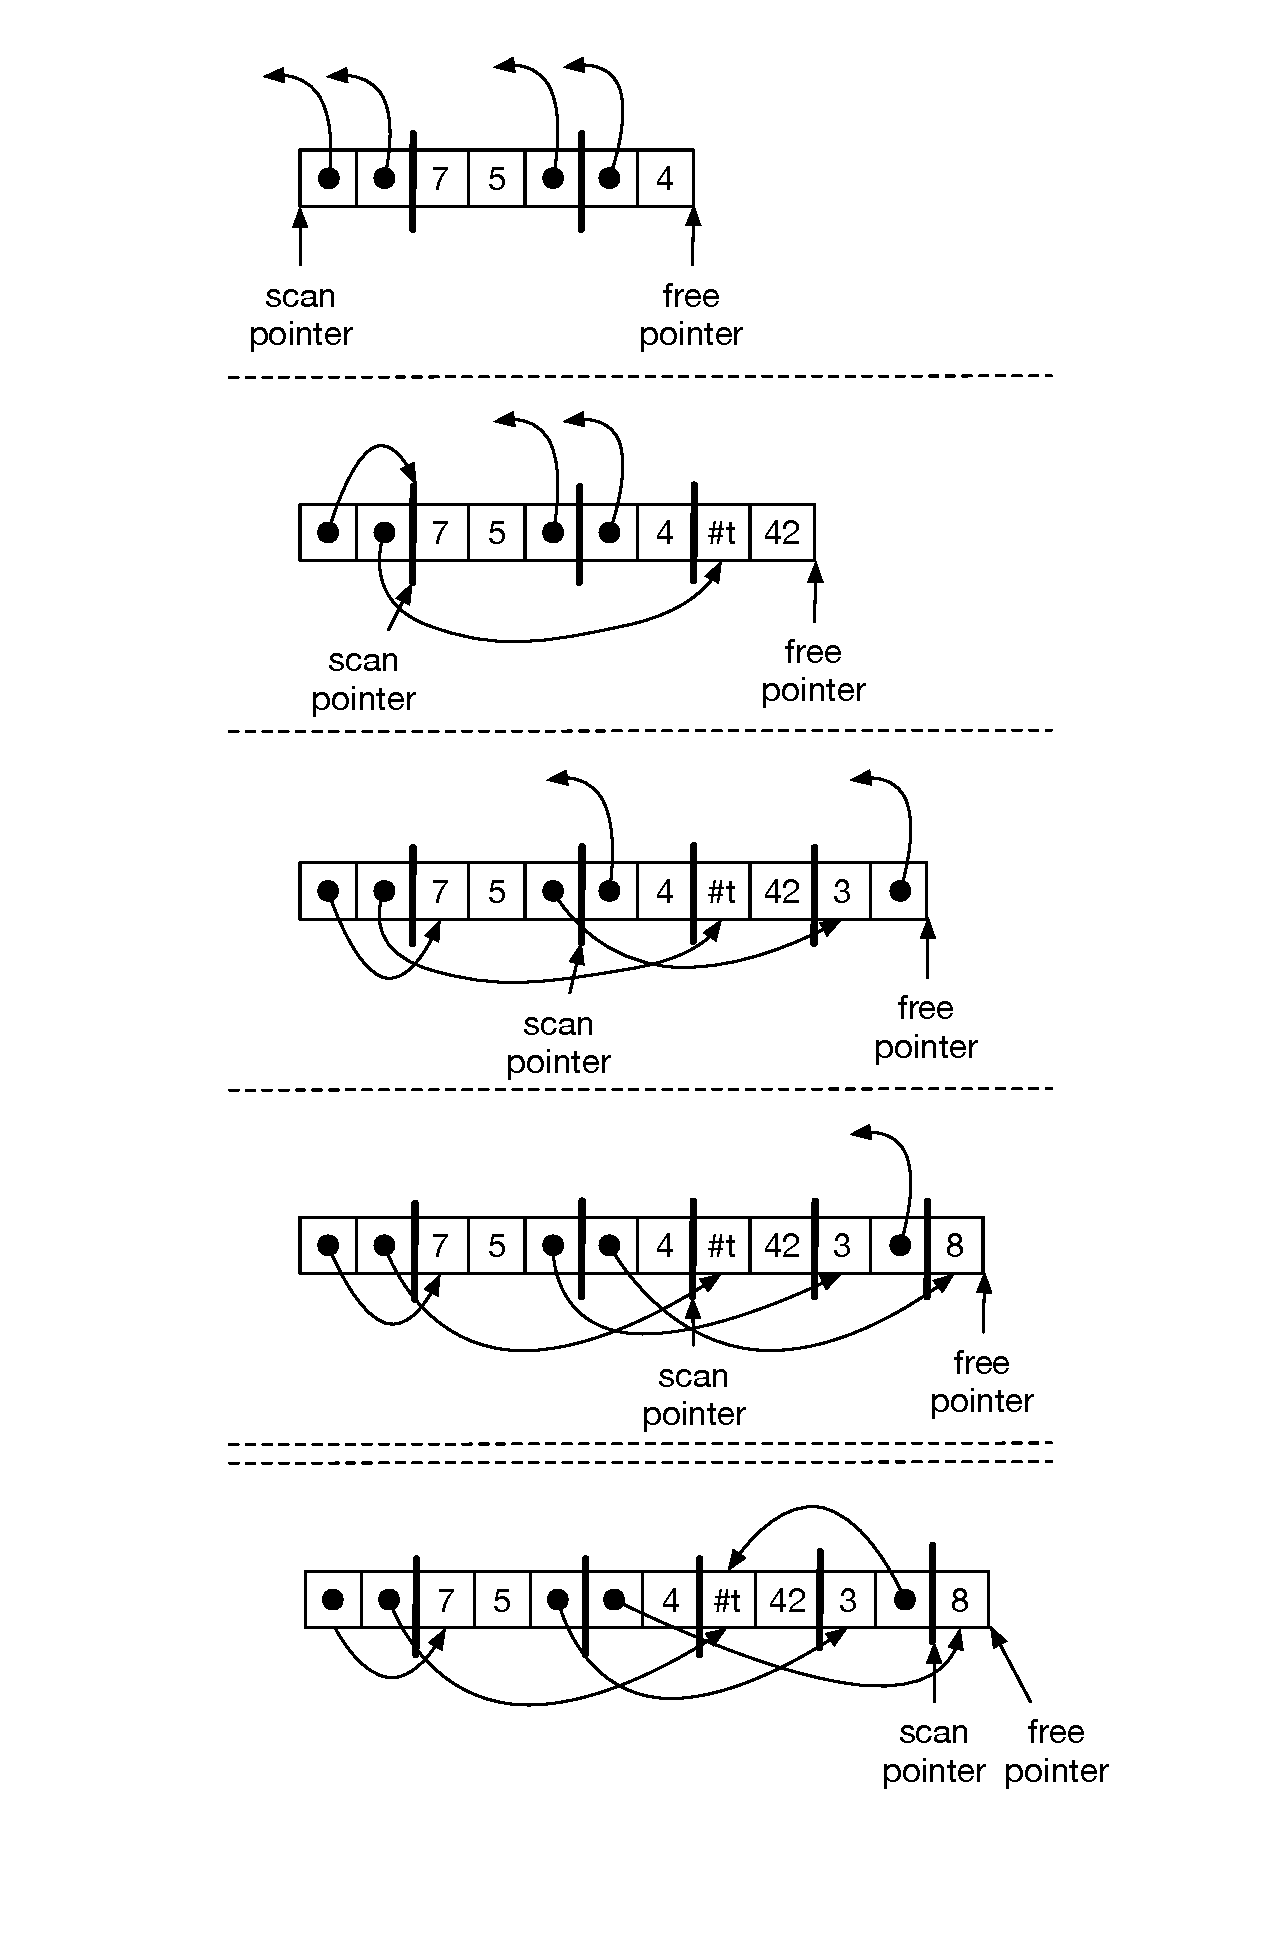
\includegraphics[width=0.9\textwidth]{figures/cheney}
\caption{拷贝回收的详细过程}
\label{fig:cheney}
\end{figure}

图\ref{fig:cheney}展示了在拷贝过程中 ToSpace 的几个瞬间。
队列由 ToSpace 开头的一块连续内存表示,使用两个指针跟踪队列的头和尾。
该算法首先将所有可以立即从根集到达的向量复制到 ToSpace 中,以形成初始队列。
当复制一个向量时,将旧向量标记为已被访问。下一小节将会讨论如何完成这个标记。
注意,队列中复制的向量内的任何指针仍然指向 FromSpace。
创建好初始队列后,算法将进入一个循环,
在循环中,算法会考察队头的向量,
将从该向量所有可以直接到达的向量复制到ToSpace并放到队尾(后移队尾指针),
然后更新队头向量中指针,使它们指向新复制的向量,
之后队头向量出队(后移队头指针),重复循环,直至队列为空,也就是队头指针赶上队尾指针。

在图\ref{fig:cheney}中,开始时队列中有三个向量。
队头向量的第一个元素指向的FromSpace中的一个被标记为已访问的向量,
这个已访问过的向量会保存它的克隆体在ToSpace中的地址(这一点在下一小节详细说明),
在这个例子中正是ToSpace中的第二个向量,因此我们把这个指针改为指向第二个向量。

队头向量的第二个元素是指向FromSpace中一个内容为\code{\#t}和\code{42}的向量,
并且它没有被标记为已访问。我们把它复制过来,放在队尾,并修改队头向量中的指针。
同时,我们还要标记FromSpace中的旧向量为已访问,
并在其中记录它的克隆体的地址(同样,见下一小节)。
此时队头向量处理完毕,我们后移队头指针,然后重复这个过程,直至队列为空。

\subsection{向量在内存中的表示}

首先,垃圾回收器需要区分指针和其他类型的数据。本文的实现策略如下:
对于指向根集的那些指针,我们不放在寄存器或者普通的过程调用栈上,
而是放在一个单独的栈上,这个栈当然也会随着函数的调用和返回相应地出栈入栈一些数据,
我们这个栈称作根栈,也叫影子栈。

而对于向量中的指针和非指针数据,我们通过在每个向量的开头增加一个额外的64位标签来实现。
图\ref{fig:tuple-rep}展示了两个示例,
注意这个图是以大端方式绘制的,从右到左,位置 0(最低位) 在最右边,
它对应着 x86 移动指令 salq (左移) 和 sarq (右移) 的方向。
“指针掩码”部分用于标记向量中哪些元素是指针,1代表为指针,0则为其他类型的数据。
指针掩码从第 7位开始,总共占 50位,因此该语言最多只允许长度为50的向量。
元组的长度 (元素的数量) 存储在位 1 到 6 的位置。
位置 0 则是我们的访问标记,如果它的值是1,则表示没有被访问,也就是还没有被复制到 ToSpace。
如果值是0,则说明这个向量已经被访问过了,
并且此时整个标签实际上是一个地址,表示的是复制后的向量在ToSpace中的位置。
(因为我们的所有数据都是64位的倍数,所以的向量8 字节对齐的,它们的地址的低 3 位总是 0。)

\begin{figure}[t]
\centering
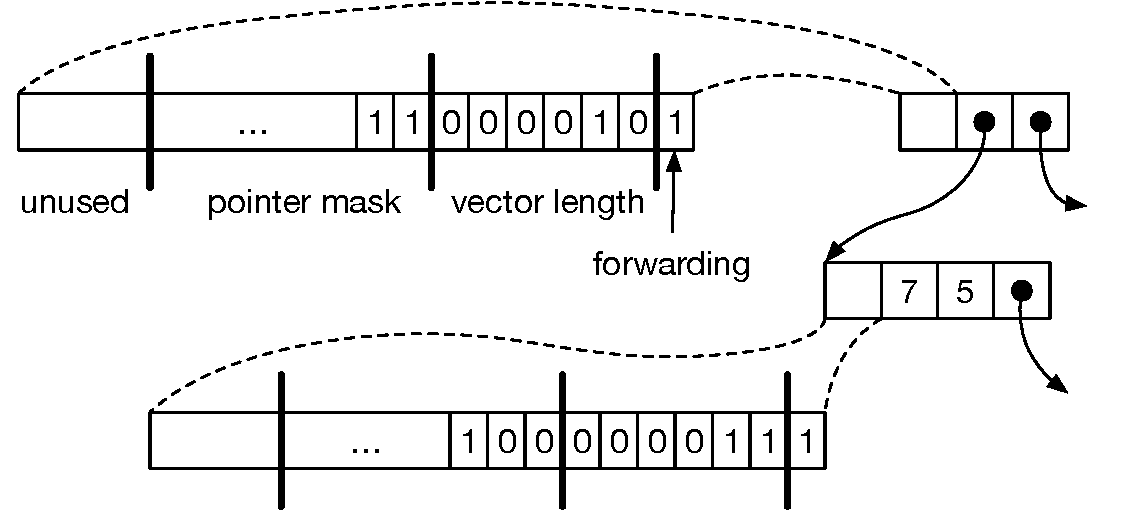
\includegraphics[width=0.8\textwidth]{figures/tuple-rep}
\caption{向量在内存中表示}
\label{fig:tuple-rep}
\end{figure}

\subsection{展开向量定义}

我们用c语言来实现垃圾回收器,编译生成一个目标文件,
和我们的编译器翻译出的汇编代码生成的目标文件一起链接成最终的可执行文件。
这个垃圾回收器提供了如下所示的几个接口。
\begin{lstlisting}
void initialize(uint64_t rootstack_size, uint64_t heap_size);
void collect(int64_t** rootstack_ptr, uint64_t bytes_requested);
int64_t* free_ptr;
int64_t* fromspace_begin;
int64_t* fromspace_end;
int64_t** rootstack_begin;
\end{lstlisting}

initialize 函数初始化 FromSpace、ToSpace 和根栈,在主函数的准备工作中被调用。
initialize 函数将 FromSpace 开头的地址放入全局变量 free\_ptr 中。
全局变量 fromspace\_end 指向的地址是 FromSpace 的最后一个元素的后面一个位置。
rootstack\_begin 变量指向根栈的第一个元素。

只要 FromSpace 中还有剩余空间,生成的代码就可以通过向前移动 free\_ptr 来分配向量。
FromSpace 中剩余的空间是 fromspace\_end 和 free\_ptr之间的差值。
当 FromSpace 中没有足够的空间留给下一次分配时,就调用 collect 函数。
collect 函数接受一个指向根栈当前顶部的指针 (栈顶元素的后面一个位置) 和需要分配的字节数。
collect 函数执行前文描述的复制回收过程。

编译器需要把一个简单的定义向量的语句翻译成一系列语句:
1) 把向量的各个元素的表达式绑定到一系列临时变量上;
2) 判断FromSpace是否有足够的空间,如果不够则调用 collect 函数;
3) 调用 allocate 函数;
4) 初始化向量。

\begin{lstlisting}
(vector |$e_0 \ldots e_{n-1}$|)
|$\Longrightarrow$|
(let ([|$x_0$| |$e_0$|]
      [|$x_{n-1}$| |$e_{n-1}$|]
      ...)
  (begin
    (if (< (+ (global-value free_ptr) |\itm{bytes}|)
           (global-value fromspace_end))
        (void)
        (collect |\itm{bytes}|))
    (let ([|$v$| (allocate |\itm{len}| |\itm{type}|)])
      (begin
        ([_ (vector-set! |$v$| |$0$| |$x_0$|)])
        ([_ (vector-set! |$v$| |$n-1$| |$x_{n-1}$|)])
        |$v$|))))
\end{lstlisting}

其中 allocate 接受参数len和向量的类型。
len指的是向量的长度,而 bytes 是需要为向量分配的总字节数,
即len加上1(一个64位的标签)再乘以8。
allocate 指令后续将被翻译为若干条汇编指令,包括根据向量的类型来计算标签的值。
